% Chapter 1

\chapter{Hardware Architecture for Inter-Prediction} % Write in your own chapter title
\label{Chapter4}
\lhead{Chapter 4. \emph{Hardware Architecture for Inter-Prediction}} % Write in your own chapter title to set the page header

There are many new technologies such as intra prediction, in-loop deblocking filter and context based arithmetic coding introduced in the latest H.264/AVC standard. Among all of these amazing technologies, \textbf{Variable Block Size Motion Estimation (VBSME)} is one of the most powerful techniques. In comparison with the previous Fixed Block Size Motion Estimation (FBSME), VBSME divides one MB into smaller blocks to fit different motion directions. In this way, the coding performance is proved.

\section{Full Search ME Algorithm}
The Full Search Algorithm works in the following way:
\begin{itemize}
	\item At first, both the search window and current block positions are fixed at the certain point i.e top left corner of frame. The current block starts the loading of the pixels from the top left corner. Absolute difference of each pixel of current block with the corresponding pixel of the search window is calculated.
	\begin{equation} \label{equ:1}
		Diff(m,n,k,l\ = |S(m+k, n+l) - C(k,l)|
	\end{equation}
	\item After that the Sum of all Absolute Differences (SAD) for that particular position of current block is calculated.
	\begin{equation} \label{equ:2}
		SAD(m,n) = \sum_{k=0}^{W-1}\sum_{l=0}^{H-1}Diff(m,n,k,l) 
	\end{equation}
	Then the current block is shifted by 1 row or column of pixels and again SAD is calculated. In this way, several SADs are calculated in a single search window.
	\item Each SAD when calculated is compared with the previous SAD value and the smaller SAD value is taken. In this way at end, minimum SAD value and the corresponding motion vectors values are depicted for one search window. 
	\begin{equation} \label{equ:3}
		SAD_{min} = min(SAD(m,n))
	\end{equation}
\end{itemize}

In the above equation (\ref{equ:1}), (\ref{equ:2}) and (\ref{equ:3}) The domain of m and n is $m \in [0, M-1] $ and $m \in [0, N-1]$ respectively.M and N are width and height of search window respectively. H and W are height and width of current block respectively. C(k,l) represents the pixel value of the current block and S(m+k, n+l) is the pixel value from the search window of the reference frame.\cite{li2003serial} \\

\section{256 PE VBS FS ME Hardware Architecture}
We designed a parallel \textbf{256 PE VBS FSME Hardware Architecture}. \cite{kalaycioglu2011low} This hardware is implemented in System Verilog. First of all, the pixels in the current MB are stored in a Block Ram \textbf{(c$\_$BRAM)}. The pixels of the search window are also stored in a block RAM \textbf{(s$\_$BRAM)}. The architecture is shown in the figure \ref{fig:256pevbsme}

\begin{figure}[H]
	\centering
	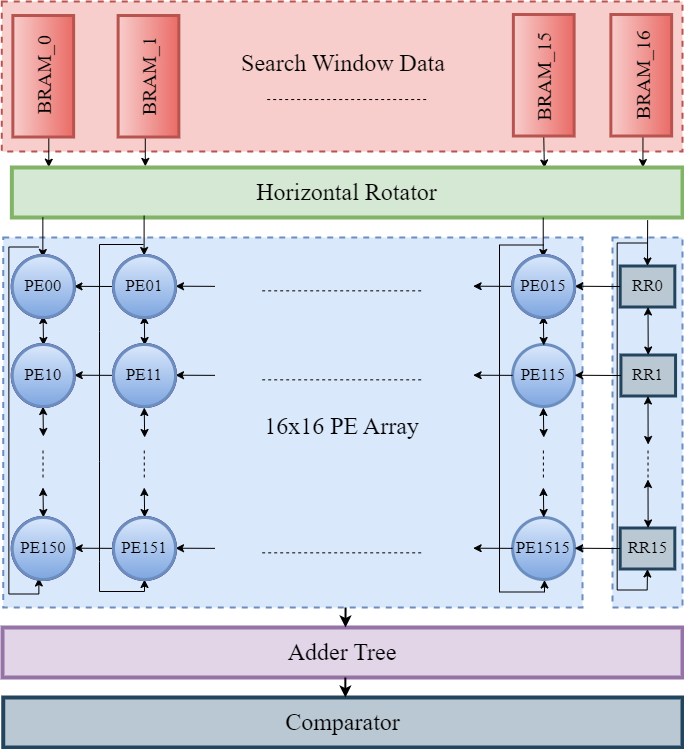
\includegraphics[width = 4in]{./Figures/256pevbsme.png}
	\rule{35em}{0.5pt}
	\caption{265 PE VBS ME Hardware Architecture}
	\label{fig:256pevbsme}
\end{figure}

In this design, a \textbf{2-D systolic PE array} is used. The use of this type of array introduced parallel computing and pipelinability in the structure. There are \textbf{16x16 = 256 PEs} ( 16 rows and 16 columns) interconnected with each other in a form of matrix. All of them are  made capable of shifting data down, up and left. It means that a 16x16 current block can move around the 48x48 search window in down, up and right direction. For a \textbf{16x16 MB}, a Motion Vector MV is found in one cycle in a search range of \textbf{[-16, 15]} pixels. Pixels are defined as 8 bit positive integers.

As soon as the control signals for loading current and search pixels are enabled, both current block and search window pixels starts loading into PEs. In 1 clock cycle, 16 pixels are loaded for both of them. (1st PE is filled in each of 16 columns). Thus, the whole PE matrix is filled in 16 cycles. As depicted in figure \ref{fig:pematrix}, \textbf{pixel$\_$cpr$\_$in} and \textbf{pixel$\_$spr$\_$in} are input array of 16 8-bit pixels from current block and search window of reference block respectively. The \textbf{pe$\_$}matrix module concatenates the output signals of each column of processing elements to form the final output signal \textbf{ad} which is an array of 8*(16**2) bits. 

\begin{figure}[H]
	\centering
	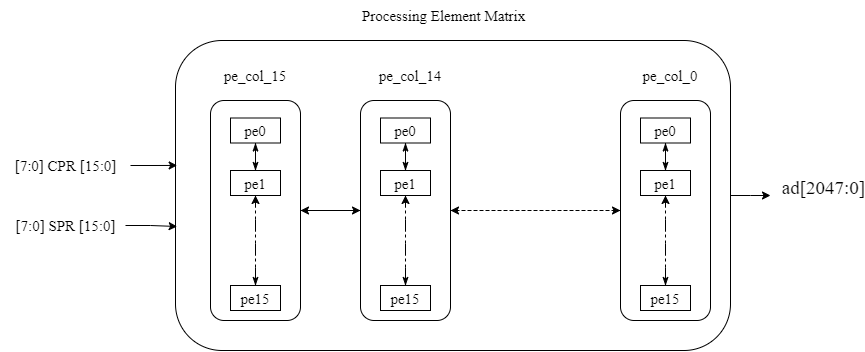
\includegraphics[width = 4.5in]{./Figures/pematrix.png}
	\rule{35em}{0.5pt}
	\caption{16 x 16 PE Matrix}
	\label{fig:pematrix}
\end{figure}

Each PE calculates the absolute difference between current MB pixel and the search window pixel. In this way 16x16 = 256 absolute differences are obtained in one location and they all are calculated simultaneously with the loading of data in PEs as the design is combinational. 

After absolute differences are all calculated, The SAD for that search location is determined by adding the absolute differences calculated by the above PEs as shown in figure. All these absolute differences are added up together using Adder Trees. The working of a simple adder tree is shown in figure \ref{fig:addertree}. It can seen clearly in the figure that there is 2 cycle latency for an adder tree. 

\begin{figure}[H]
	\centering
	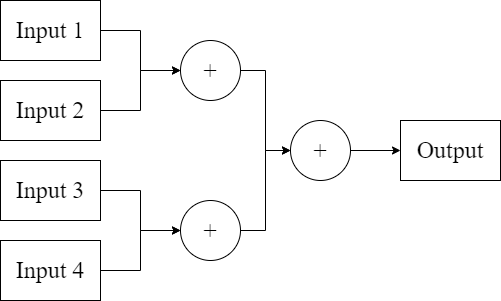
\includegraphics[width = 2in]{./Figures/addertree.png}
	\rule{35em}{0.5pt}
	\caption{Working of an Adder Tree}
	\label{fig:addertree}
\end{figure}

\subsection{PI-PPSAD Architecture for SAD Calculation}

For SAD calculation of a 16x16 current block, we consider \textbf{PI-PPSAD} structure. The current pixels adn reference pixels are broadcasted into the respective PE arrays. This is shown by the vertical dash lines in the figure \ref{fig:pippsad}. Each row of PE determines the absolute difference with one row in macro block. One row SAD gets accumulated with partial SAD propagated in, which belongs to the same search position. After that, the result is propagated to the next stage in vertical.

\begin{figure}[H]
	\centering
	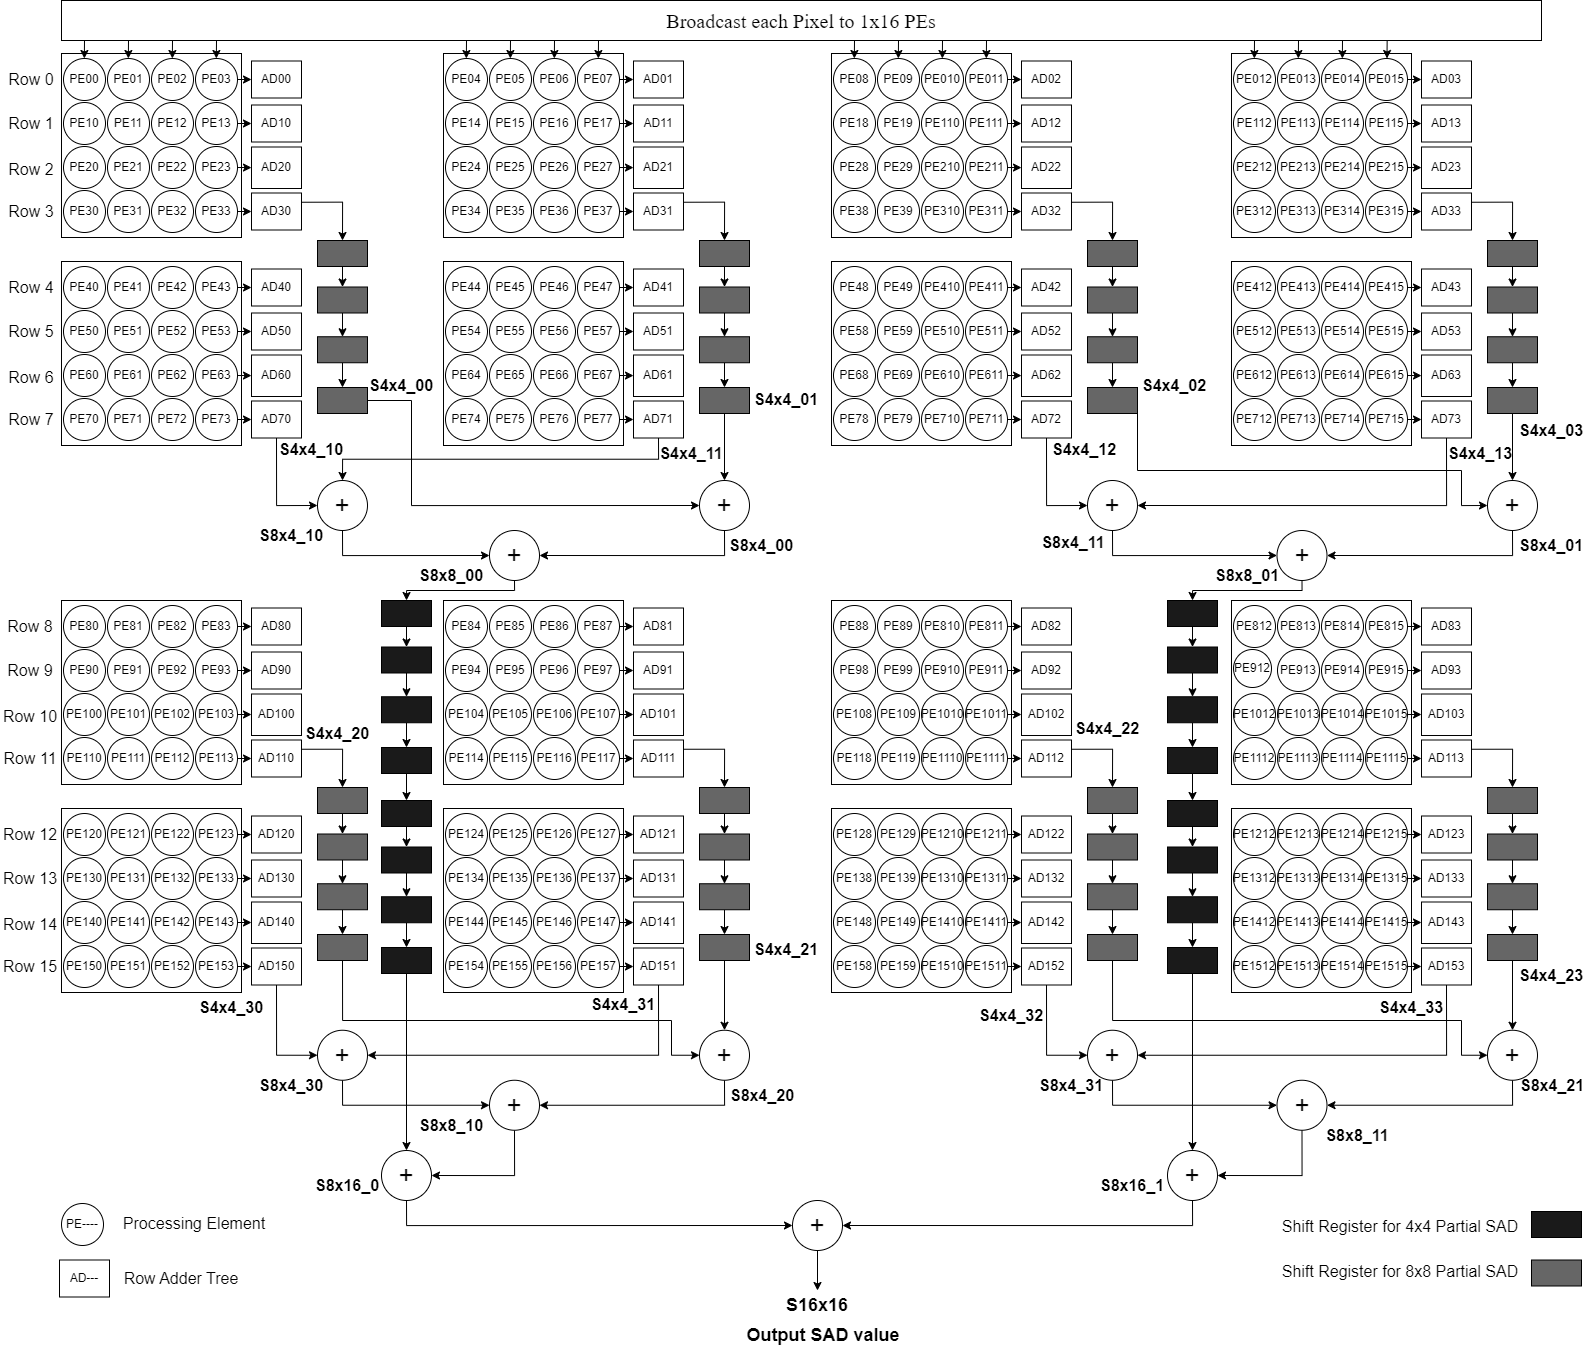
\includegraphics[width = 5.5in]{./Figures/PIPPSAD.png}
	\rule{35em}{0.5pt}
	\caption{PI-PPSAD Architecture}
	\label{fig:pippsad}
\end{figure}

In out Pi-PPSAD architecture, when the output of seventh PE row is obtained, inside one macro-Block, the SADs of the upper half partitions which include S4x4$\_$YX (Y: 0-1 X: 0-3), S8x4$\_$YX (Y: 0-1 X: 0-1), S8x8$\_$0X (X: 0-1), they are depicted through one adder tree. In order to calculate S8x16$\_$0, S8x16$\_$1 and S16x16, the SADs of S8x8$\_$00 and S8x8$\_$01 are continue to be transmitted by making the use of shift registers. At the last stage of pipeline, they are summed with SADs of S8x8$\_$10 and S8x8$\_$11 to compute S8x16$\_$0, S8x16$\_$1 and the final SAD value depicted as S16x16 for that specific position of current and search block. This process is shown in figure \ref{fig:pippsad}.

The previous architecture of PI$\_$PPSAD or PPSAD model as described in \cite{huang2003hardware}, it propagates all the 4x4 SAD to the through the pipline. At the last stage of pipline, these partial 4x4 SADs sum up to generate other SADs. If we compare the design in our project with this previous design, it propagates 8x8 partial SADs in last stages of pipeline. In this way, the hardware cost for this data propagation is reduced. Approximately, 560-bit registers can be saved. The maximum path delay is made short as the operand number to the adder tree is reduced. Previously, the critical path lies in the adder tree of last stage. As it had to calculated SAD direct from 4x4 block SADs, so the input number of adder tree was 16. But in the proposed design, we first use 8 4x4 block SADs and the 2 8x8 block SADs as the operands to the ast adder tree, so the operand number is reduced to 10. In this way, minimum delay is reduced and complex circuit of adder tree is simplified. Moreover, the latency for the blocks in upper half of macro blocks is reduced from 16 to 8 cycles. This latency is in such a way that one clock cycle for synchronous reading from BRAM, one clock cycle for horizontal shifting, one clock cycle for SAD computation in a 2D systolic PE array, two clock cycles for the adder tree to generate 4x4 SADs, and three clock cycles for the adder tree to generate 41 MVs for seven different block sizes.

Initially, pipelining causes latency of 16 cycles in the SAD calculation. But, once the pipeline is filled, only one cycle is needed per SAD value. Current block data is loaded only once when the current block is changed while search are pixels are fed in every cycle to the PEs. Their data flow is further explained in table \ref{tab:dataflow1} and \ref{tab:dataflow2}. As, there are 48 columns of reference pixels search range window [-16,15]. Thus, per 16x16 macro block, the approximate number of cycles is 48*32 = 1536 cycles. \cite{lin2008parallel}

\subsection{Zig-Zag Search Pattern}

The proposed hardware searches the search locations in a 48x48 search window in a zig-zag pattern as shown in figure \ref{fig:zigzag}. Usually most of the proposed ME architectures with 256 PEs make use of vertical search flow i.e start from top left corner and when end of the column is reached, the search location at top of the next column is searched. Thus, 
we have to either broadcast multiple pixels into the PEs or delay all the PEs until they are filled every time when we reach the end of the column and move to the top of the next \cite{hardware_architecture_design}.

\begin{figure}[H]
	\centering
	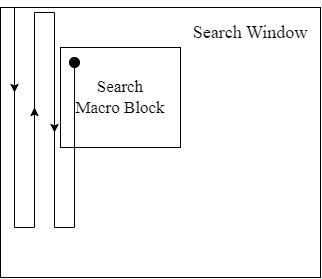
\includegraphics[width = 2in]{./Figures/zigzag.png}
	\rule{35em}{0.5pt}
	\caption{Zig-Zag Search Pattern}
	\label{fig:zigzag}
\end{figure}

The zig-zag architecture used in our implementation can referred from \cite{fast_vlsi_architecture}. But, this structure either use both row and column aligned memories or use data duplication. The implemented architecture overcomes this problem by introducing pipeline of 16 8-bit temporary registers. The search starts from top left corner of the search window and continues downwards until the last search location of this column is searched. After that, current block shifts to one right column in a way that pixel columns are shifted one left. Thus the search proceeds with the last search location of this next column and continues upwards until the first search location is reached. Only 16 new search window pixels are required by the current block PE array in each cycle to calculate the SAD of the next search location not keeping in fact its position in the search window. \cite{kalaycioglu2011low} 


\subsection{Data Flow in 256 PEs}

Data flow of PEs for fixed location of a current marco block pixels while searching all the locations in search window is shown in table \ref{tab:dataflow1} and \ref{tab:dataflow2} where sw(x,y) are the search window pixels.

When iterating the search locations in the 1$^{st}$ column of search window, vertical up shift is performed in the PE array in each cycle. All PEs are provided the search window pixels from their neighboring PEs except for those PEs in the last row. These last row PEs read 16 new search window pixels from 16 BRAMs in each cycle. The 17$^{th}$ BRAM help in performing left shift after all search locations in a column has been searched. It is connected to temporary registers. When there is the need for left shift, the pixels need for the right most PEs become ready in those temporary registers. When we are done with the searches in the first 16 columns, a left shift is performed in the PE array and the PEs in the 16$^{th}$ column receive search window pixels from temporary registers. \cite{kalaycioglu2011low}

\begin{table}[H]
	\centering
	\begin{tabular}{|c|c|c|c|c|c|c|c|c|c|c|}
		\hline
		
		\textbf{Clock} &  \multicolumn{4}{c|}{\textbf{1$^{st}$ Column}} &  \multicolumn{4}{c|}{\textbf{2$^{nd}$ Column}} & \\
		
		\cline{2-9}
		
		& \textbf{PE(0,15)} & \textbf{PE(0,14)} & ... & \textbf{PE(0,0)} & \textbf{PE(1,15)} & \textbf{PE(1,14)} & ... & \textbf{PE(1,0)} & ... \\
		
		\hline
		0 & sw(0,0) & none & ... & none & sw(1,0) & none & ... & none & ... \\
		
		1 & sw(0,1) & sw(0,0) & ... & none & sw(1,1) & sw(1,0) & ... & none & ... \\
		
		... & ... & ... & ... & ... & ... & ... & ... & ... & ... \\
		
		14 & sw(0,14) & sw(0,13) & ... & none & sw(1,14) & sw(1,13) & ... & none & ... \\
		
		15 & sw(0,15) & sw(0,14) & ... & sw(0,0) & sw(1,15) & sw(1,14) & ... & sw(1,0) & ... \\
		
		\hline
		
		16 & sw(0,16) & sw(0,15) & ... & sw(0,1) & sw(1,16) & sw(1,15) & ... & sw(1,1) & ... \\
		
		17 & sw(0,17) & sw(0,16) & ... & sw(0,2) & sw(1,17) & sw(1,16) & ... & sw(1,2) & ... \\
		
		... & ... & ... & ... & ... & ... & ... & ... & ... & ... \\
		
		45 & sw(0,45) & sw(0,44) & ... & sw(0,30) & sw(1,45) & sw(1,44) & ... & sw(1,30) & ... \\
		
		46 & sw(0,46) & sw(0,45) & ... & sw(0,31) & sw(1,46) & sw(1,45) & ... & sw(1,31) & ... \\
		
		\hline
		
		47 & sw(1,46) & sw(1,45) & ... & sw(1,31) & sw(2,46) & sw(2,45) & ... & sw(2,31) & ... \\
		
		48 & sw(1,45) & sw(1,44) & ... & sw(1,30) & sw(2,45) & sw(2,44) & ... & sw(2,30) & ... \\
		
		... & ... & ... & ... & ... & ... & ... & ... & ... & ... \\
		
		77 & sw(1,16) & sw(1,15) & ... & sw(1,1) & sw(2,16) & sw(2,15) & ... & sw(2,1) & ... \\
		
		78 & sw(1,15) & sw(1,14) & ... & sw(1,0) & sw(2,15) & sw(2,14) & ... & sw(2,0) & ... \\
		
		\hline
		
		1007 & sw(31,46) & sw(31,45) & ... & sw(31,31) & sw(32,46) & sw(32,45) & ... & sw(32,31) & ... \\
		
		1008 & sw(31,45) & sw(31,44) & ... & sw(31,30) & sw(32,45) & sw(32,44) & ... & sw(32,30) & ... \\
		
		... & ... & ... & ... & ... & ... & ... & ... & ... & ... \\
		
		1037 & sw(31,16) & sw(31,15) & ... & sw(31,1) & sw(32,16) & sw(32,15) & ... & sw(32,1) & ... \\
		
		1038 & sw(31,15) & sw(31,14) & ... & sw(31,0) & sw(32,15) & sw(32,14) & ... & sw(32,0) & ... \\
		
		\hline
	\end{tabular}
	\caption{ Data Flow of PEs in 256PE VBS ME Hardware (a)}
	\label{tab:dataflow1}
\end{table}

Once left shift is performed, in each cycle, vertical down shift is performed and all the PEs are provided search window pixels from their neighbouring PEs except the PEs in the 1$^{st}$ row.  These 1$^{st}$ row PEs read 16 new search window pixels from 16 BRAMs. This search pattern of data flow is also depicted in figure \ref{fig:zigzag}. There total 17 BRAMs and each BRAM store pixels in every 17$^{th}$ column of the search window. The 1$^{st}$ BRAM stores pixels in 1$^{st}$, 18$^{th}$ and 35$^{th}$ olumns, 2$^{nd}$ BRAM fills in 2$^{nd}$, 19$^{th}$ and 36$^{th}$ columns and so the rest of BRAMs. The search window pixels which are read from the BRAMs have static order. But, the search window pixels that are required by PE array and temporary registers, the order for them varies depending on the columns being processed. Horizontal rotator hardware solve this problem by reordering the 16+1 pixels in a search macro block.

\begin{table}[H]
	\centering
	\begin{tabular}{|c|c|c|c|c|c|c|c|c|c|}
		\hline
		\textbf{Clock} &  &  \multicolumn{4}{c|}{\textbf{16$^{th}$ Column}} &  \multicolumn{4}{c|}{\textbf{Temp Column}}  \\
		\cline{3-10}
		& ... & \textbf{PE(15,15)} & \textbf{PE(15,14)} & ... & \textbf{PE(15,0)} & \textbf{reg 15} & \textbf{Reg 14} & ... & \textbf{Reg 0}  \\
		\hline
		0 & ... & sw(15,0) & none & ... & none & sw(16,0) & none & ... & none  \\
		
		1 & ... & sw(15,1) & sw(15,0) & ... & none & sw(16,1) & sw(16,0) & ... & none  \\
		
		... & ... & ... & ... & ... & ... & ... & ... & ... & ... \\
		
		14 & ... & sw(15,14) & sw(15,13) & ... & none & sw(16,14) & sw(16,13) & ... & none \\ 
		
		15 & ... & sw(15,15) & sw(15,14) & ... & sw(15,0) & sw(16,15) & sw(16,14) & ... & sw(16,0)  \\
		
		\hline
		
		16 & ... & sw(15,16) & sw(15,15) & ... & sw(15,1) & sw(16,16) & sw(16,15) & ... & sw(16,1) \\
		
		17 & ... & sw(15,17) & sw(15,16) & ... & sw(15,2) & sw(16,17) & sw(16,16) & ... & sw(16,2) \\
		
		... & ... & ... & ... & ... & ... & ... & ... & ... & ... \\
		
		45 & ... & sw(15,45) & sw(15,44) & ... & sw(15,30) & sw(16,45) & sw(16,44) & ... & sw(16,30) \\
		
		46 & ... & sw(15,46) & sw(15,45) & ... & sw(15,31) & sw(16,46) & sw(16,45) & ... & sw(16,31)  \\
		
		\hline
		
		47 & ... & sw(16,46) & sw(16,45) & ... & sw(16,31) & sw(17,46) & sw(17,45) & ... & sw(17,31) \\
		
		48 & ... & sw(16,45) & sw(16,44) & ... & sw(16,30) & sw(17,45) & sw(17,44) & ... & sw(17,30) \\
		
		... & ... & ... & ... & ... & ... & ... & ... & ... & ... \\
		
		77 & ... & sw(16,16) & sw(16,15) & ... & sw(16,1) & sw(17,16) & sw(17,15) & ... & sw(17,1) \\
		
		78 & ... & sw(16,15) & sw(16,14) & ... & sw(16,0) & sw(17,15) & sw(17,14) & ... & sw(17,0)  \\
		
		\hline
		
		1007 & ... & sw(46,46) & sw(46,45) & ... & sw(46,31) & none & none & ... & none \\
		
		1008 & ... & sw(46,45) & sw(46,44) & ... & sw(46,30) & none & none & ... & none \\
		
		... & ... & ... & ... & ... & ... & ... & ... & ... & ... \\
		
		1037 & ... & sw(46,16) & sw(46,15) & ... & sw(46,1) & none & none & ... & none \\
		
		1038 & ... & sw(46,15) & sw(46,14) & ... & sw(46,0) & none & none & ... & none  \\
		
		\hline
	\end{tabular}
	\caption{ Data Flow of PEs in 256PE VBS ME Hardware (b)}
	\label{tab:dataflow2}
\end{table}

 Out of all the SADs that are being calculated during this searching, the minimum value and its corresponding motion vectors are depicted as output. This task is performed by comparator which compares the upcoming SAD value with the previously stored minimum value. After comparison, minimum one is depicted as output This type of Architecture requires large area and a lot of hardware implementation but the performance rate is high due to number of parallel computation and use of pipeline structure.